
%(BEGIN_QUESTION)
% Copyright 2014, Tony R. Kuphaldt, released under the Creative Commons Attribution License (v 1.0)
% This means you may do almost anything with this work of mine, so long as you give me proper credit

Dette cross-limited luft/drivstoff-forholdsreguleringssystemet skal holde drivstoff/luft-forholdet på 1:1 ved alle fyringsnivåer. Anta at det har fungert korrekt lenge på 30\% fyringsrate (dvs. fyringskommando = 30\%; luftflow = 30\%; drivstoffflow = 30\%):

$$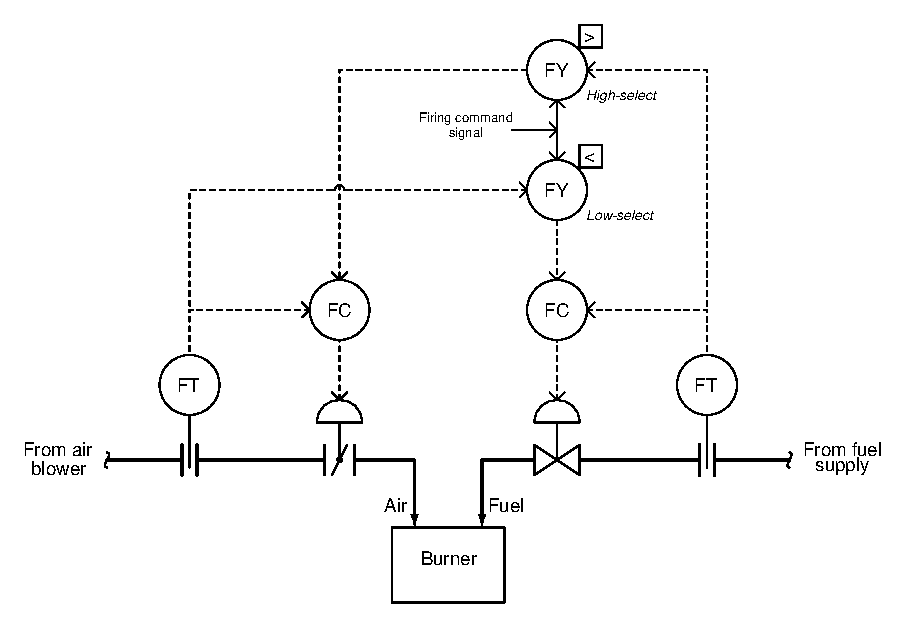
\includegraphics[width=15.5cm]{i00934x01.eps}$$

\noindent
Velg det beste svaret som beskriver umiddelbar effekt på prosessen dersom luftflowtransmitteren plutselig feiler med {\it lavt} signal:

\begin{itemize}
\item{} Brennerens drivstoff/luft-blanding blir {\it rik} (for mye drivstoff i forhold til luft)
\vskip 10pt
\item{} Brennerens drivstoff/luft-blanding blir {\it mager} (for mye luft i forhold til drivstoff)
\vskip 10pt
\item{} Både luft- og drivstoffventil stenger, slik at brenneren slukker
\vskip 10pt
\item{} Både luft- og drivstoffventil åpner 100\%, slik at brenneren går til maks effekt
\end{itemize}

\underbar{file i00934}
%(END_QUESTION)





%(BEGIN_ANSWER)

Brennerens drivstoff/luft-blanding blir {\it mager} (for mye luft i forhold til drivstoff)

%(END_ANSWER)





%(BEGIN_NOTES)

{\bf Denne oppgaven er ment kun for eksamen, ikke for arbeidsark!}.

%(END_NOTES)

